\nonstopmode
%\documentclass[11pt]{article}
\documentclass[runningheads]{llncs}

\usepackage{amsmath,amssymb,mathtools}
%\usepackage{amsthm}
%\usepackage{fullpage}
\usepackage{xspace}
\usepackage{color,soul}
\usepackage{paralist}

% \usepackage[linesnumbered, ruled]{algorithm2e}

\usepackage[final]{microtype}
\usepackage[final]{hyperref}
\usepackage{subcaption}

% DEBUG
%\usepackage{lipsum}
%\usepackage{todonotes}
%\usepackage{lineno}
%\linenumbers

% EXTRA
%\usepackage{authblk}

\usepackage{tikz}
\usetikzlibrary{
	arrows,
	arrows.meta,
	calc,
	patterns,
	positioning,
	shapes,
	decorations.pathmorphing,
	decorations.markings,
	decorations.pathreplacing,
	quotes,
}

% \usetikzlibrary{graphs, graphdrawing}
% \usegdlibrary{trees,force,layered}

\tikzset{
	>=Latex, 
	on grid, 
	auto, 
	thick,
	->,
}

% NODE
\tikzset{default node/.style={
	draw, 
	circle,
	inner sep=0mm,
	minimum size=5mm,
	very thick,
	font=\small,
	black!70,
}}

\tikzset{clear node/.style={
	draw=none, 
	inner sep=0mm,
	minimum size=0mm,
}}

% LABELS
\tikzset{label/.style={
	shape=rectangle,
	draw=none,
	sloped,
	midway,
}}

\tikzset{label above/.style={
	label,
	above=.5mm,
}}

\tikzset{label below/.style={
	label,
	below=.5mm,
}}

% EDGES
\tikzset{
	light/.style={
		thin,
		gray,
	},
	path/.style={
		light,
		decorate, 
		decoration={snake, segment length=18pt},
	},
	brace/.style={
		decorate,
		decoration={brace, amplitude=5},
		-,
	},
}

\tikzset{cloud/.style={
	path,
	-,
	decoration={snake, segment length=24pt},
}}

% MISC
\tikzset{group/.style={
	dotted, 
	semithick, 
	orange, 
	-
}}

\renewcommand{\floatpagefraction}{0.6}

\sloppy


%%%%%%%%%%%%%%%%%%%%%%%%%%%%%%%%%%%%%%%%%%%%%%%%%%%%%%%%%%%%%%%%%%%%%

%% handy commands

\newcommand{\eqdf}{\stackrel{\scriptscriptstyle \triangle}{=}}
\newcommand{\argmin}{\ensuremath{\mbox{argmin}}}
\newcommand{\argmax}{\ensuremath{\mbox{argmax}}}
\newcommand{\set}[1]{\left\{ #1 \right\}}
\newcommand{\paren}[1]{\left( #1 \right)}
\newcommand{\bit}{\set{0,1}}
\newcommand{\inv}[1]{\frac{1}{#1}}
\newcommand{\abs}[1]{\left| #1 \right|}
\newcommand{\ceil}[1]{\left\lceil {#1} \right\rceil}
\newcommand{\floor}[1]{\left\lfloor {#1} \right\rfloor}
\newcommand{\half}{\frac{1}{2}}
\newcommand{\threehalves}{\frac{3}{2}}

\newcommand{\naturals}{\mathbb{N}}
\newcommand{\rationals}{\mathbb{Q}}
\newcommand{\reals}{\mathbb{R}}
\newcommand{\integers}{\mathbb{Z}}

\newcommand{\eps}{\varepsilon}

%%%%%%%%%%%%%%%%%%%%%%%%%%%%%%%%%%%%%%%%%%%%%%%%%%%%%%%%%%%%%%%%%%%%%

\newcommand{\scp}{\textsc{SCP}\xspace}
\newcommand{\scplong}{\textsc{Service Chain Placement}\xspace}

\newcommand{\calE}{\mathcal{E}}
\newcommand{\calG}{\mathcal{G}}
\newcommand{\calV}{\mathcal{V}}

\newcommand{\dror}[1]{\sethlcolor{yellow}\hl{Dror: #1}}

\def\R{\mathbb{R}}
\def\N{\mathbb{N}}


%%%%%%%%%%%%%%%%%%%%%%%%%%%%%%%%%%%%%%%%%%%%%%%%%%%%%%%%%%%%%%%%%%%%%

\title{\bf Service Chain Placement in SDNs%
\thanks{Research supported in part by Network Programming (Neptune)
  Consortium, Israel.}
}

\titlerunning{Service Chain Placement in SDNs}


%\author[1]{Gilad Kutiel%
%\thanks{E-mail: \texttt{gkutiel@cs.technion.ac.il}}}

%\author[2]{Dror Rawitz%
%\thanks{Partially supported by the Israel Science Foundation
%  (grant no.~497/14).  E-mail: \texttt{dror.rawitz@biu.ac.il}}}

%\affil[1]{Department of Computer Science, Technion, Haifa, Israel}
%\affil[2]{Faculty of Engineering, Bar Ilan University, Ramt-Gan, Israel}

\author{%
Gilad Kutiel
\and
Dror Rawitz%
\thanks{Partially supported by the Israel Science Foundation
  (grant no.~497/14).  }
}

\institute{%
Department of Computer Science, Technion, Haifa 32000, Israel. \\
\email{gkutiel@cs.technion.ac.il}
\and
Faculty of Engineering, Bar Ilan University, Ramt-Gan 52900, Israel.\\
\email{dror.rawitz@biu.ac.il}
}

%%%%%%%%%%%%%%%%%%%%%%%%%%%%%%%%%%%%%%%%%%%%%%%%%%%%%%%%%%%%%%%%%%%%%

\begin{document}
\maketitle

\begin{abstract}
We study the allocation problem of a request for a \emph{service
chain} in a software-defined network that supports network function
virtualization.
%
Given a network that contains servers with limited processing power
and of links with limited bandwidth, a service chain is a sequence of
virtual network functions (VNFs) that service a certain flow request
in the network.
%
The allocation of a service chain consists of routing and VNF
placement.  That is, each VNF from the seqeunce is placed in a server
along a path, and it is feasible if each server can handle the VNFs
that are assigned to it, and if each link on the path can carry the
flow that is assigned to it.
%
A request for service is composed of a source and a destination in the
network, an upper bound on the total latency, and a specification of
all service chains that are considered valid for this request.
%
In addition, each pair of server and VNF are associated with a cost
for placing the network function in the server.  Given a request, the
goal is to find a valid service chain of minimum total cost that
respects the latency constraint or to identify that such a service
chain does not exist.

We show that even the feasibility problem is NP-hard in general
graphs.  Hence we focus on directed acyclic graphs (DAGs).  We show
that the problem is still NP-hard in DAGs even for a very simple
network, and even if the specification consists of only one option.
%
On the other hand, we present an FPTAS for the case where the network
is a DAG and the specification is also represented as a DAG.  Based on
our FPTAS, we provide a randomized algorithm for instances in which
the service chain passes through a bounded number of servers whose
degree is larger than two.
\end{abstract}

%%%%%%%%%%%%%%%%%%%%%%%%%%%%%%%%%%%%%%%%%%%%%%%%%%%%%%%%%%%%%%%%%%%%%

\section{Introduction}


Computer communication networks are in constant need of expansion to
cope with the ever growing traffic.  As networks grow, management and
maintenance become more and more complicated.
%
Current developments aim to improve the utilization of network
resources include the detachment of network applications from network
infrastructure and the transition from network planning to network
programming.

One aspect of network programming is to manage resources from a
central point of view, namely to make decisions based on availability,
network status, required quality of service, and the identity of the
client.  Hence, a focal issue is a central agent that is able to
received reports from network components and client requests, and as a
result can alter the allocation of resources in the networks.  This
approach is called Software Defined Networking (SDN), where there is a
separation between routing and management (control plane) and the
underlying routers and switches that forward traffic (data plane) (see
Kreutz et al.~\cite{KRVRAU15}).

A complimentary approach is Network Function Virtualization
(NFV)~\cite{NFV12}.  Instead of relying on special purpose machines,
network applications become virtual network functions (VNF) that are
executed on generic machines and can be placed in various locations in
the network.  Virtualization increases the flexibility of resource
allocation and thus the utilization of the network resources.
%
Internet Service Providers (ISPs) that provide services to clients
benefit from NFV, since it helps to better utilize their physical
network.  In addition, when network services are virtualized, an ISP
may support \emph{service chaining}~\cite{ServiceChaining15}, namely a
compound service that consists of a sequence of VNFs.  Furthermore,
one may offer a compound service a service that may be obtained using
one of several sequences of VNFs.




%%%%%

\paragraph*{\bf Related work.}
%

Cohen et al.~\cite{CLNR15} considered VNF placement.  In their model
the input is an undirected graph with a metric distance function on
the edges.  clients are located in various nodes, and each client is
interested in a subset of VNFs.  For each node $v$ and VNF $\alpha$,
there is a setup cost associated with placing a copy of $\alpha$ at
$v$ (multiple copies are allowed), and there is a load that is induced
on $v$ for placing a copy of $\alpha$.  Furthermore, each node has a
limited capacity.  Also, each copy of a VNF can handle a limited
amount of clients A solution is the assignment of each client to a
subset of nodes, each corresponding to one of its required VNFs.  The
cost of a solution is the total setup costs plus the sum of distances
between the clients and the node from which they get service.
%
Cohen et al.~\cite{CLNR15} gave bi-criteria approximation algorithms
for various versions of the problem, namely algorithms that compute
constant factor approximations that violate the load constraints by a
constant factor.
%
It is important to note that in this problem the authors do not consider
routing, and also it assumes unordered VNF subsets.

Even, Medina, and Patt-Shamir~\cite{EMP16} studied online path
computation and VNF placement.  They considered compound requests that
arrive in an online manner.  Each request is a flow with a
specification of routing and VNF requirements.  The specification is
represented by a DAG whose vertices are VNFs.  Each VNF can be
performed by a specified subset of servers in the system.  Upon
arrival of a request, the algorithm either rejects the request or
accepts it with a specific routing and VNF assignment, under given
server capacity constraints.  Each request has a benefit that is
gained if it is accepted, and the goal is to maximize the total
benefit gained by accepted requests.
%
Even, Medina, and Patt-Shamir~\cite{EMP16} proposed an algorithm that
copes with requests with unknown duration without preemption by using
a third response, which is refer to as “stand by”, whose competitive
ratio is $O(\log (knb_{\max})$, where $n$ is the number of nodes,
$b_{\max}$ is an upper bound on a request benefit per time unit, and
$k$ is the maximum number of VNFs of any service chain.  This
performance guarantee holds for the case where the processing of any
request in any possible service chain is never more than
$O(1/(k \log (nk)))$ fraction of the capacity of any network
component.
%
Even, Rost, and Schmid~\cite{ERS16} presented a randomized
approximation algorithm for the same problem that computes
$(1-\eps)$-approximate placements if the processing of any processing
request in any possible service chain is never more than
$O(\eps^2/\log n)$ fraction of the capacity of any network component.

\dror{add references - see [ERS16]}

\paragraph*{\bf Our results.}
%
In this paper we study the allocation problem of a compound flow
request for a service chain in a software-defined network that
supports NFV, where the goal is to find an optimal placement with
respect to the current available resources from the point of view of
the network (i.e., the ISP).
%
More specifically, we consider the case where the network already
contains previous resource allocations.  Therefore, we are given a
(physical) network that contains servers with limited (residual)
processing power and of links with limited (residual) bandwidth.
%
A request for service is composed of a source and a destination in the
network, an upper bound on the total latency, and a specification of
all service chains that are considered valid for this request.  As
in~\cite{EMP16}, the specification is represented by a DAG whose
vertices are VNFs.
%
The allocation of a service chain consists of routing and VNF
placement.  That is, each VNF from the sequence is placed in a server
along a path, and it is feasible if each server can handle the VNFs
that are assigned to it, and if each link on the path can carry the
flow that is assigned to it.  Moreover each link causes a delay, and
the service chain placement should also comply with a bound on the
total latency.
%
Each pair of server and VNF are associated with a cost for placing the
network function in the server.  This cost measures compatibility of a
VNF to a server (e.g., infinite costs means ``incompatible'').  Given
a request, the goal is to find a feasible service chain of minimum
total cost or to identify that a valid service chain does not exist.

We show that the feasibility problem is NP-hard in general graphs
using a reduction from \textsc{Hamiltonian Path}.  Hence we focus on
directed acyclic graphs (DAGs).  We show that the problem is still
NP-hard in DAGs even for a very simple network, and even if the
specification consists of only one option.  Both reductions are from
the \textsc{Partition} problem.
%
On the positive side, we present an FPTAS for the case where the
network is a DAG.  Based on our FPTAS, we provide a randomized
algorithm for instances in which the service chain passes through a
bounded number of servers whose degree is larger than two.


%%%%%%%%%%%%%%%%%%%%%%%%%%%%%%%%%%%%%%%%%%%%%%%%%%%%%%%%%%%%%%%%%%%%%

\section{Preliminaries}


\paragraph*{\bf Model.}
%
The \scplong (\scp) input is composed of three components, a physical
network, a virtual specification, and placement costs:
\begin{description}
\item[Physical network:]
%
  The physical network is a digraph $G = (V,E)$.  Each node $v \in V$
  has a non-negative processing capacity $p(v)$, and each directed
  edge $e \in E$ has a non-negative bandwidth cap $b(e)$.

\item[Virtual specification:]
%
  The description of a request for a service chain consists of a
  physical source $s \in V$, a physical destination $t \in V$, and a
  directed acyclic graph (DAG) $\calG = (\calV,\calE)$.
%
  Without loss of generality, we assume that $p(s) = p(t) = 0$.  
%
  The DAG $\calG$ has a source node $\sigma \in \calV$ and a
  destination $\tau \in \calV$. Each node $\alpha \in \calV$ represent
  a VNF that has a processing demand $p(\alpha)$.  Without loss of
  generality, we assume that $p(\sigma) = p(\tau) = 0$.  Each edge
  $\eps \in \calE$ has a bandwidth demand $b(\eps)$.
  
\item[Placement costs:]
%
  There is a non-negative cost $c(\alpha,v)$ for placing the VNF
  $\alpha$ in $v$.  We assume that $c(\sigma,s) = 0$ and $c(\sigma,v)
  = \infty$, for every $v \neq s$.  Similarly, we assume that
  $c(\tau,t) = 0$ and $c(\tau,v) = \infty$, for every $v \neq t$.
\end{description}

A solution consists of the following:
\begin{description}
\item[Virtual path:] A path from $\sigma$ to $\tau$ in $\calG$, namely
  a sequence of vertices $\alpha_0,\ldots,\alpha_q$, where
  $\alpha_0 = \sigma$, $\alpha_q = \tau$, and
  $(\alpha_j,\alpha_{j+1}) \in \calE$, for every $j \in
  \set{0,\ldots,q-1}$.

\item[Physical path:] A simple path from $s$ to $t$ in $G$, namely a
  sequence of node $v_0,\ldots,v_k$, where $v_0 = s$, $v_k = t$, and
  $(v_i,v_{i+1}) \in E$, for every $i \in \set{0,\ldots,k-1}$.
  
\item[Placement:] A function $f$ that maps the virtual path to the
  physical path.  Formally, a placement is a function $f:
  \set{\alpha_0,\ldots,\alpha_q} \to \set{v_0,\ldots,v_k}$
  such that
\begin{enumerate}
\item If $f(\alpha_j) = v_i$ and $f(\alpha_{j+1}) = v_{i'}$, then $i
  \leq i'$.
\item $b(\alpha_j,\alpha_{j+1}) \leq b(v_i,v_{i+1})$, for every
  $(v_i,v_{i+1}) \in \bar{f}(\alpha_j,\alpha_{j+1})$, where
  $\bar{f}(\alpha_j,\alpha_{j+1})$ to be the set of physical edges
  that correspond to it, i.e.,
\[
\bar{f}(\alpha_j,\alpha_{j+1}) \eqdf \set{(v_i,v_{i+1}) : i' \leq i < i''}
~,
\]
  where $f(\alpha_j) = v_{i'}$ and $f(\alpha_{j+1}) = v_{i''}$.

\item $\sum_{\alpha \in f^{-1}(v)} p(\alpha) \leq p(v)$, where
  $f^{-1}(v) \eqdf \set{\alpha : f(\alpha) = v}$.
 
\end{enumerate}
\end{description}

An example of an \scp instance and a solution is given in
Figure~\ref{fig:solution}.

\begin{figure}
\centering
\scalebox{1}{
\begin{tikzpicture}[every node/.style={default node}, very thick]

\begin{scope}[random seed=1, spring layout, node distance=1.8cm]
\node(a) {a};
\node(b) {b};
\node(c) {c};
\node(d) {d};
\node(e) {e};
\node(f) {f};
\node(g) {g};
\node(h) {h};
\node(i) {i};
\node(j) {j};

\graph{
	(a) -> (b);
	(b) -> {(d), (e)};
	(d) -> {(f), (h)};
	(f) -> {(g), (h), (c)};
	(h) -> {(g), (i), (e)};
	{[edges={blue, dashed}]
		(a) -> (c) -> (d) -> (e) -> (i) -> (g) -> (j);
	}
};

\node(pa) {a'};
\node(pb) {b'};
\node(pc) {c'};
\node(pd) {d'};
\node(pe) {e'};
\node(pf) {f'};
\node(pg) {g'};
\node(ph) {h'};

\graph{
	(pa) -> (pb);
	(pb) -> {(pd), (pe)};
	(pd) -> {(pf), (ph)};
	(pf) -> {(pg), (ph), (pc)};
	(ph) -> {(pg), (pe)};
	(pe) -> (ph);
};
\end{scope}

\begin{scope}[dotted, orange, -]
\draw
(a.north east) to[out=135, in=45] node(j1)[midway, clear node] {}
(c.north west) to[out=225, in=135]
(d.south west) to[out=-45, in=-45]
(a.north east)
;

\draw
(e.east) to[out=-90, in=-90] node(j2)[midway, clear node] {}
(i.west) to[out=90, in=90]
(e.east)
;

\draw
(g.east) to[out=-90, in=-90] node(j3)[midway, clear node] {}
(j.west) to[out=90, in=90]
(g.east)
;

\draw[->] (j1) to[bend left] (pa);
\draw[->] (j2) to[bend right] (pe);
\draw[->] (j3) to[bend right] (pg);
\end{scope}
	

\node[clear node] at(-5,0) {Virtual Graph};
\node[clear node] at(5, -2){Physical Graph};

\end{tikzpicture}
}
\caption{???}
\label{fig:solution}
\end{figure}

The cost of a placement $f$ is:
\[
\sum_j c(\alpha_j,f(\alpha_j))
~.
\]
In \scp the goal is to find a feasible placement of a virtual path
into the physical DAG that minimizes the cost.

%%%%%

We also consider an extended version of \scp in which each physical
link causes a delay and there is an upper bound $L$ on the total
delay.  More formally, each pair of a virtual edge $\eps$ and physical
edge $e$ is associated with a latency $\ell(\eps,e)$.
%
Given a placement $f: \set{\alpha_0,\ldots,\alpha_q} \to
\set{v_0,\ldots,v_k}$, the total latency of the solution is given by
\[
L(f) = \sum_j \sum_{e \in \bar{f}(\eps)} \ell(\eps,e)
~.
\]
In this case there is an additional constraint that $L(f) \leq L$.


%%%%%

\paragraph*{\bf Definitions and notation.}
%
Define $n_p \eqdf \abs{V}$ and $m_p \eqdf \abs{E}$.  Similarly, define
$n_v \eqdf \abs{\calV}$ and $m_v \eqdf \abs{\calE}$.

Given a virtual DAG $\calG$, we assume the existence of a topological
sorting of the vertices and write $\alpha \prec \beta$ if $\alpha$
precedes $\beta$ in this ordering.  If the physical network is a DAG,
then we make a similar assumption and write $v \prec u$ if $v$
precedes $u$ in this ordering.


%%%%%%%%%%%%%%%%%%%%%%%%%%%%%%%%%%%%%%%%%%%%%%%%%%%%%%%%%%%%%%%%%%%%%

\section{Hardness Results}

In this section we present three hardness results.  First, we show
that even the feasibility question of \scp is NP-hard, and therefore
no approximation algorithm exists for \scp.  In addition, we show that
\scp is NP-hard even if $\abs{V \setminus \set{s,t}} = 1$.  We also
show that \scp is NP-hard even if both the physical network and the
virtual DAG are simple paths.

We start by showing that even finding a feasible solution is NP-hard.

\begin{theorem}
Feasibility of \scp is NP-hard
\end{theorem}
\begin{proof}
We use a reduction from \textsc{Hamiltonian Path} that is known to be
NP-hard~\cite{GarJoh79}.
%
Given an instance $H$ of \textsc{Hamiltonian Path} we construct an
instance of \scp.  For the physical network we have that $G$, where
$V(G) = V(H) \cup \set{s,t}$, and $E(G) = E(H) \cup \set{(s,v),(v,t) :
  v \in V(H)}$.  In addition, $p(v) = 1$, for every $v$, and $b(e) =
1$, for every $e$.  The virtual DAG $\calG$ is a path containing $n+2$
virtual functions, $\sigma = \alpha_0, \alpha_1, \ldots, \alpha_n,
\alpha_{n+1} = \tau$, where $p(\alpha_i) = 1$, for every $i \in
\set{1,\ldots,n}$.  Also, $b(\alpha_i,\alpha_{i+1}) = 1$, for every
$i$.

The construction can clearly be computed in polynomial time.
%
An Hamiltonian Path in $G$, induces a \scp solution that follows the
path, i.e., $\alpha_i$ is placed in the $i$th vertex along the path.
%
One the other hand, since all demands and capacities are $1$, no two
VNFs can share a physical node.  Hence a \scp solution induces an
Hamiltonian path.
%
\qed
\end{proof}

Next, we show that \scp is NP-hard even if the physical network is
very simple. 

\begin{theorem}
\label{thm:simple}
\scp is NP-hard, even if $\abs{V \setminus \set{s,t}} = 1$.
\end{theorem}
\begin{proof}
We prove the theorem using a reduction from \textsc{Partition}.
Given a \textsc{Partition} instance $a = \set{a_1, \ldots, a_n}$ we
construct an \scp instance as follows.
%
The physical network $G$ contains three nodes: $s$, $v$, and $t$, and
there are two edges $(s,v)$ and $(v,t)$.  The capacity of $v$ is $p(v)
= \half \sum_i a_i$.  Edge bandwidth are zero.
%
The virtual DAG is composed of $2n+2$ vertices, namely
\[
\calV
= \set{\sigma,\tau}
  \cup \set{\alpha_1, \ldots, \alpha_n}
  \cup \set{\beta_1, \ldots, \beta_n}
~.
\]
Also,
\[
\calE
= \bigcup_i \set{ \set{\alpha_i,\beta_i} \times \set{\alpha_{i+1},\beta_{i+1}} } 
  \cup
  \set{ (\sigma,\alpha_1), (\sigma,\beta_1), (\alpha_n,t), (\beta_n,t) }
~.
\]
The DAG is shown in Figure~\ref{fig:simple}.
%
The demands are $p(\alpha_i) = a_i$ and $p(\beta_i) = 0$, for every
$i$.  Also, $b(\eps) = 0$, for every $\eps \in \calE$.  The costs are:
$c(\alpha_i,v) = 0$ and $c(\beta_i,v) = a_i$, for every $i$.

The \scp instance can be computed in polynomial time.
%
Also, it is not hard to verify that $a \in \textsc{Partition}$ if and
only if there exists a solution whose cost is $\half \sum_i a_i$.
%
\qed
\end{proof}

\begin{figure}[t]
\centering
\begin{tikzpicture}[every node/.style={default node}, very thick]

\begin{scope}[layered layout, grow=right, sibling distance=2cm, level distance=2cm]

\node(v1p) {$v_1^+$};
\node(v1m) {$v_1^+$};
\node(v2p) {$v_2^-$};
\node(v2m) {$v_2^-$};
\node[clear node, inner sep=5mm](dotsp) {$\ldots$};
\node[clear node, inner sep=5mm](dotsm) {$\ldots$};
\node(vnp) {$v_n^-$};
\node(vnm) {$v_n^-$};



\graph{
	s -> {(v1p), (v1m)};
	(v1p) -> {(v2p), (v2m)};
	(v1m) -> {(v2p), (v2m)};
	(v2p) -> {(dotsp), (dotsm)};
	(v2m) -> {(dotsp), (dotsm)};
	(dotsp) -> {(vnp), (vnm)};
	(dotsm) -> {(vnp), (vnm)};
	{(vnp), (vnm)} -> t;
};

\end{scope}

\end{tikzpicture}

\caption{The specification defined in the proof of Theorem~\ref{thm:simple}.}
\label{fig:simple}
\end{figure}

Next, we show that \scp is NP-hard even if both the physical network
and the VNF specification are paths.

\begin{theorem}
\scp is NP-hard, even if both the physical network and the virtual DAG
are paths.
\end{theorem}
\begin{proof}
The prove the theorem using a reduction from \textsc{Partition}.
Given a \textsc{Partition} instance $\set{a_1, \ldots, a_n}$, we
construct a virtual path $\sigma, \alpha_1, \ldots, \alpha_n, \tau$
and a physical path $s, v_1^-, v_1^+, \ldots, v_n^-, v_n^+, t$.  We
set $p(v) = 1$, for every node $v \neq s,t$, and $p(\alpha_i) = 1$,
for every $i$.  In addition, we set $b(e) = 1$, for every edge $e \in
E$, and $b(\eps) = 1$, for every edge $\eps \in \calE$.
%
As for the costs, we define $c(\alpha_i, v_i^-) = 0$, $c(\alpha_i,
v_i^+) = a_i$, and for any $v \notin \{v_i^-,v_i^+\}$ we set
$c(\alpha_i, v) = \infty$.  We also define $\ell((\alpha_i,\alpha_{i+1}),
(v_i^-,v_i^+)) = a_i$, and set $\ell(\eps,e) = 0$, otherwise.  Finally,
we set $L = \half \sum_i^n a_i$.
%
Figure~\ref{fig:reduction2} depicts the above reduction.

One can easily verify that $a_i$ is either counted in the latency of in the cost.
Hence, 
$\set{a_1, \ldots,
a_n} \in \textsc{Partition}$ if and only if there is a placement with
cost $\half \sum_i^n a_i$.
%
\qed
\end{proof}


\begin{figure}[t]
\centering
\scalebox{.9}{
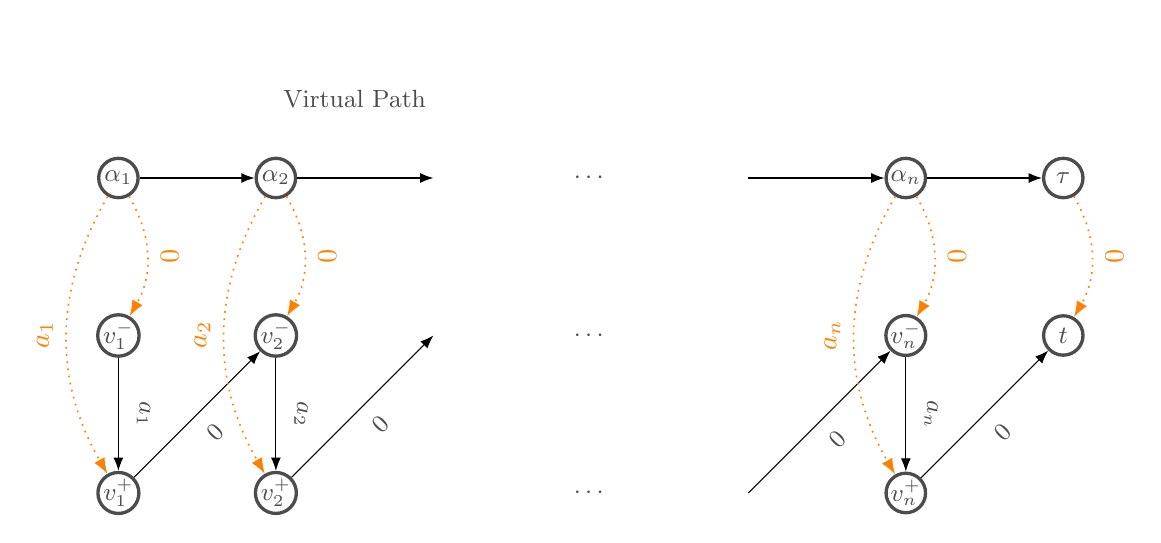
\begin{tikzpicture}[every node/.style={default node}]
\node[draw=none] at(3, 1) {Virtual Path};

\node(alpha1) at(0,0) {$\alpha_1$};
\node(alpha2) at(2,0) {$\alpha_2$};
\node[draw=none] at(6,0) {$\cdots$};
\node(alphan) at(10,0) {$\alpha_n$};
\node(tau) at(12,0) {$\tau$};

\draw (alpha1) -- (alpha2);
\draw (alpha2) -- +(2, 0);
\draw ($(alphan) + (-2,0)$) -- (alphan);
\draw (alphan) -- (tau);

\node(v1-) at(0, -2) {$v_1^-$};
\node(v1+) at(0, -4) {$v_1^+$};
\node(v2-) at(2, -2) {$v_2^-$};
\node(v2+) at(2, -4) {$v_2^+$};

\node[draw=none] at(6,-2) {$\cdots$};
\node[draw=none] at(6,-4) {$\cdots$};

\node(vn-) at(10, -2) {$v_n^-$};
\node(vn+) at(10, -4) {$v_n^+$};
\node(t) at(12, -2) {$t$};

\draw (v1-) -- (v1+) node[label above] {$a_1$};
\draw (v1+) -- (v2-) node[label below] {$0$};
\draw (v2-) -- (v2+) node[label above] {$a_2$};
\draw (v2+) -- +(2, 2)node[label below] {$0$};

\draw ($(vn-) + (-2,-2)$) -- (vn-)node[label below] {$0$};;
\draw (vn-) -- (vn+)node[label above] {$a_n$};
\draw (vn+) -- (t)node[label below] {$0$};;

\begin{scope}[every node/.style={label above, orange}]
\draw[group, ->] (alpha1) to[bend left] node {$0$} (v1-);
\draw[group, ->] (alpha1) to[bend right] node {$a_1$} (v1+);
\draw[group, ->] (alpha2) to[bend left] node {$0$} (v2-);
\draw[group, ->] (alpha2) to[bend right] node {$a_2$} (v2+);
\draw[group, ->] (alphan) to[bend left] node {$0$} (vn-);
\draw[group, ->] (alphan) to[bend right] node {$a_n$} (vn+);

\draw[group, ->] (tau) to[bend left] node {$0$} (t);
\end{scope}

\end{tikzpicture}

}
\caption[]{
\label{fig:reduction2}
A reduction from a partition instance $a_1, \ldots, a_n$.
The cost function enforces each $\alpha_i$ to be placed either 
in $v_i^-$ or in $v_i^+$.
In the former case this placement incure no cost but additional latency of $a_i$,
in the later case there will be additional $a_i$ cost with zero latency.
}
\end{figure}


%%%%%%%%%%%%%%%%%%%%%%%%%%%%%%%%%%%%%%%%%%%%%%%%%%%%%%%%%%%%%%%%%%%%%

\section{Algorithms}
\label{sec:algorithms}

%%%%%

\subsection{???}

In this section, 
assuming costs are integral and polynomial bounded in the input length,
we present an efficient algorithm to \scp{}.
We then extend the algorithm to also obey a global latency constraint.
Finally we argue that, using a standard scaling and rounding technique, we can use
the same computation to achieve a solution with a cost only
$1 + \varepsilon$ times greater that of the optimal solution, for any
$\varepsilon > 0$, i.e. an FPTAS, for an arbitrary cost function.
These are recursive algorithms that can be efficiently implemented using
dynamic programming.

We are given an instance of the \scp{} problem 
$
\calG = (\calV, \calE),
G = (V, E),
(\sigma , \tau , s, t),
(p, b, c)
$.
The algorithm maintains a pair of physical and virtual nodes,
$\gamma$ and $w$ respectively.
In each step it chooses a virtual edge $\alpha\beta$ and a physical node $v$
that are ascendant of $\gamma$ and $w$ respectively.
It then embeds a minimum cost $\beta\gamma$-path into $w$ 
without violating its processing capacity,
it also compute a $vw$-path to be used in the solution, 
making sure the path can carry the bandwidth demand of the edge $\beta\gamma$.
Finally it finds an optimal embedding to a $\sigma\alpha$-path into a $sv$-path 
recursively.
This informal description of the algorithm is illustrated in Figure~\ref{fig:dp1}.

\begin{figure}[t]
\centering
\begin{tikzpicture}[every node/.style={default node}]
\node[draw=none] at(5, 2.7) {Virtual Graph};

\node(sv) at(0,0) {$\sigma$};
\node(v0) at(4,0) {$\alpha$};
\node(v1) at(6.5,1) {$\beta$};
\node[draw=none] at(6.5,0) {$\vdots$};
\node(v3) at(6.5,-1) {};
\node(tv) at(10,0) {$\gamma$};

\draw[cloud, blue, dashed] 
($(sv.west) + (-.3,0)$)	to[out=90, in=90] 
($(v0.east) + (.3, 0)$)	to[out=-90, in=-90]
($(sv.west) + (-.3,0)$)
;

\draw (v0) -- (v1) node[label above] {$b_d(\alpha\beta)$};
\draw[dashed] (v0) -- (v3);

\draw[path] (v1) -- (tv.north west);
\draw[path] (v3) -- (tv.south west);

\draw[brace, light] ($(v0) + (-.5, 1.6)$) -- ($(tv) + (.5, 1.6)$)
node[label above, above=2mm] {\small min cost path}
;


\node[draw=none] at(4.5, -8) {Physical Graph};
\node(s) at(0,-5) {s};
\node(p1) at(5, -4){u};
\node[draw=none] at(5, -5){$\vdots$};
\node(p3) at(5, -6){};
\node(t) at(7.5,-5) {v};

\draw[cloud, blue, dashed] 
($(s.west) + (-.3,0)$)			to[out=85, in=150] 
($(p1.north east) + (.3, 0)$)	to[out=-90, in=90]
($(p3.south east) + (.3, 0)$)	to[out=210, in=-85]
($(s.west) + (-.3,0)$)
;

\draw (p1) -- (t) node[label above] {$b_c(uv)$};
\draw (p3) -- (t);

\draw[group]
(v1.west) to[out=90, in=180]
(v1.north) to[out=0, in=135]
(tv.north east) to[out=-45, in=0]
(tv.south) to[out=180, in=-45] coordinate[near start](f)
(v1.south west) to[out=135, in=-90]
(v1.west)
;

\draw[group, ->] (f) to[bend left] (t.east);
\end{tikzpicture}
\caption[]{
\label{fig:dp1}
The optimal embedding of a $\sigma \gamma $-path into a $sw$-path can be
efficiently computed by breaking the problem into the problem of embedding 
a $\sigma\alpha$-path into a $sv$-path (blue, dashed rectangles) 
and the problem of embedding a $\beta\gamma$-path into $w$ (orange, dotted).
The $vw$-path must carry $b(\alpha\beta)$ bandwidth, 
The $\beta\gamma$-path is a minimum cost $\beta\gamma$-path 
that can be embedded into $w$.
}
\end{figure}

We now give a more formal description of the algorithm.
Let $C(\sigma-\gamma , s-w)$ denote the
minimum cost embedding of a $\sigma\gamma $-path into a $sw$-path.
Also let $C(\beta-\gamma, w)$ be the minimum cost
embedding of a $\beta\gamma$-path into $w$, 
and let $r_b(v, w)$ be a predicate that is true if $w$ is reachable from $v$
using only edges with bandwidth at least $b$. 
We claim that $C$ can be computed recursively as follow:
\begin{align*}
&C(\sigma-\gamma , s-w) = 
\min_{\substack{
\alpha\beta \in \calE,  
v \in V:
\\
v \prec w,
\\
\beta \prec \gamma, 
\\
r_{b(\alpha\beta)}(v,w)
}}
C(\sigma-\alpha , s-v)
+
C(\beta-\gamma, w)
\\
&C(\sigma-\sigma , s-v) = 0
\\
&C(\sigma-\alpha , s-s) = \infty
\end{align*}
Computing $C(\sigma-\tau , s-t)$ gives the optimal embedding. 
It is clear that $r_b(v,w)$ can be computed efficiently by removing all the edges
with bandwidth less than $b$ and checking connectivity.
We now argue that $C(\beta-\gamma, w)$ can be computed efficiently as well.
Let $P_w(\alpha-\gamma, c)$ 
be the minimum processing required to embed a virtual, 
$\alpha\gamma$-path into $w$ with a cost constraint $c$, 
then $P$ can be computed recursively as follow:
\begin{align*}
&P_{w}(\alpha-\gamma, c) = 
\min_{\beta\gamma  \in \calE} P_{w}(\alpha-\beta, c - c(\gamma, w))
\\
&P_w(\alpha-\alpha, c) = 
\begin{cases}
p(\alpha) & c(\alpha, w) \leq c
\\
\infty & \text{otherwise}
\end{cases}
\\
&P(\cdot, \cdot, <0) = \infty
\end{align*}
To complete our argument observe that the following holds:
$$C(\beta-\gamma, w) = \smashoperator{\min_{c : P_w(\beta-\gamma, c) \leq p(w)}}c$$ 

%%%%%

\subsection{???}

We now consider the \scp{} problem with latency.
Recall that in this variant of the problem we are also given a latency function
$l : E \times \calE \to \R$, and a latency constraint $T$.
The goal is to find a minimum cost embedding that also respect the latency
constraint.

We first describe an algorithm that, given a cost constraint $c$, 
finds an embedding that costs at most $c$ and has the minimum possible latency.
Once again, the algorithm maintains a pair of physical and virtual nodes,
$\gamma$ and $w$ respectively.
In each step it chooses a virtual edge $\alpha\beta$ and a physical node $v$
that are ascendant of $\gamma$ and $w$ respectively.
It then finds a $vw$-path that support the bandwidth of $\alpha\beta$ and
has the minimum possible latency with respect to this edge.
It also finds $\beta\gamma$-path that can be embedded into $w$ and has the 
minimum possible cost.
Finally it finds an embedding of a $\sigma\alpha$-path into a $sv$-path with 
the minimum possible latency recursively.

Let $L(\sigma-\gamma, s-w, c)$ denote an embedding of a $\sigma\gamma$-path
into a $sw$-path with the minimum possible latency that cost at most $c$.
Let $L(\alpha\beta, v-w)$ be the minimum possible latency on a $\alpha\beta$-path
w.r.t virtual edge $\alpha\beta$, using only edges with bandwidth capacity at
least $b(\alpha\beta)$, i.e. $\forall_{e \in \bar{f}(\alpha\beta)}~b(e) \geq
b(\alpha\beta)$, and $\sum_{e \in \bar{f}(\alpha\beta)}l(\alpha\beta, e)$ is
minimum.
Observe that the later can be reduced to a shortest path problem on $G$ by removing
edged with bandwidth less than $b$ and setting the weight of each edge $e$ to be 
$l(\alpha\beta, e)$.
Now $L(\sigma-\gamma, s-w, c)$ can be computed recursively as follow:
\begin{align*}
&L(\sigma-\gamma, s-w, c) = 
\min_{\substack{
\alpha\beta \in \calE,  
v \in V:
\\
v \prec w,
\\
\beta \prec \gamma, 
\\
r_{b(\alpha\beta)}(v,w)
}}
L(\alpha\beta, v-w) + 
L(\sigma-\alpha, s-v, c - C(\beta-\gamma, w))
\\
&L(\sigma-\sigma, s-v, \geq 0) = 0
\\
&L(\sigma-\alpha, s-s, \cdot) = \infty
\\
&L(\cdot, \cdot, <0) = \infty
\end{align*} 

Now, to compute the optimal embedding with the additional latency constraint,
$T$, one can simply (binary) search for the minimum value of $c$ such that
$L(\sigma-\tau, s-t, c) \leq T$.

%%%%%

\subsection{???}

To conclude this section we show that for an arbitrary cost function, $c$,
and for any $\varepsilon > 0$ 
we can defined a scaled, rounded function $c'$ such that:
\begin{enumerate}
\item $OPT_{c'} \leq (1 + \varepsilon)OPT$, where $OPT_{c'}$ is the optimal
value w.r.t $c'$ and $OPT$ is the optimal value w.r.t $c$.
\item $\max_{\alpha, v : c'(\alpha, v) \neq \infty}c'(\alpha, v)$ is polynomial
bounded in the size of the input.
\end{enumerate}
Note that combining the above claim with the algorithms described
earlier yields FPTAS for the \scp{} problem for an arbitrary cost function.

Let $\hat{c}$ be the maximum cost incurs by embedding a single virtual node into 
a physical node in an optimal embedding, 
that is $\hat{c} \eqdf \max_{\alpha \in \calV}c(\alpha, f_{opt}(\alpha))$.
Given $\varepsilon$ we define 
$$
c'(\alpha, v) \eqdf
\begin{cases}
\ceil{c(\alpha, v)/\mu} & c(\alpha, v) \leq \hat{c}
\\
\infty & c(\alpha, v) > \hat{c}
\end{cases}
$$
where 
$
\mu \eqdf \frac{\hat{c}\varepsilon}{n}
$.
Let $s$ be an optimal placement w.r.t $c'$ 
and let $o$ be an optimal placement w.r.t $c$, 
let also $S$ and $O$ denotes their values respectively, then.
\begin{lemma}
S \leq (1 + \varepsilon)O
\end{lemma}
\begin{proof}
\begin{align*}
S = & \sum_{\alpha \in \calV}c(\alpha, s(\alpha)) \leq
\\&
\mu\sum_{\alpha \in \calV}c'(\alpha, s(\alpha)) \leq
\\&
\mu\sum_{\alpha \in \calV}c'(\alpha, o(\alpha)) \leq
\\&
\mu\sum_{\alpha \in \calV}c(\alpha, o(\alpha))/\mu + 1 \leq
\\&
\sum_{\alpha \in \calV}c(\alpha, o(\alpha)) + n\mu =
O + \hat{c}\varepsilon \leq (1 + \varepsilon)O
\end{align*}
\end{proof}
Clearly, $\hat{c}$, is not known in advanced, but one can "guess" 
its value as there are at most
$|\calV| \cdot |V|$ possible values to choose from.


%%%%%%%%%%%%%%%%%%%%%%%%%%%%%%%%%%%%%%%%%%%%%%%%%%%%%%%%%%%%%%%%%%%%%

\section{General Graphs}
\label{sec:general}

In this section we consider the problem when the physical network is undirected.
Once again we seek to embed a virtual $\sigma\tau$-path 
into a simple physical $st$-path.
Note, that we still assume that the virtual graph is a DAG. 
We extend our algorithm to work for this case as well.

Recall that the problem on general graphs cannot be approximate at all,
thus we assume in this section that there exists an optimal embedding that uses
a physical path with at most $k$ \emph{heavy} vertices, thus are vertices with
degree greater than two (we do not assume anything about the physical network).
The modified algorithm includes a preprocessing stage that applies
random orientation to the physical network, the entire algorithm runs in
$O(t(n)k!)$, where $t(n)$ is the time it takes to compute the optimal embedding when the
physical network is a DAG, and finds the optimal embedding with high
probability.

The preprocessing stage is as follow:
let $V_h$ be the set of heavy vertices, and let 
$\pi:V_h \to [|V_h|]$ be a random permutation.
For every \emph{light path} $w_1, \ldots, w_l$, that is, $w_1, w_l \in
V_h$, $\pi(w_1) < \pi(w_l)$, and $\forall_{1 < i < l}, w_i \notin V_h$,
we direct the edges from $w_1$ to $w_l$ i.e. $w_i \to w_{i+1}$ for every $1
\leq i \leq l - 1$.
One can verifies that this can be done efficiently and that when this process
terminates $G$ is a DAG, Figure~\ref{fig:orientation} depicts the preprocessing
stage.

\begin{figure}[ht]
\input{fig-orientation}
\caption{
\label{fig:orientation}
The preprocessing stage: on the left is the undirected physical network,
Only the heavy nodes are drawn.
The numbers represent the permutation and the blue, dashed path represents a
path of an optimal embedding.
On the right side is the orientated physical network, 
note that it is enough that the internal ordering of the nodes on the blue,
dashed path is "correct" to ensure that the algorithm finds the optimal
embedding. }
\end{figure}

Completing the orientation, we use our previous algorithm to find an optimal
embedding.
We repeat this process, each time with a new independent random permutation, and
keep the best embedding so far.
Note that if there is an optimal embedding using a physical path with at most
$k$ heavy vertices then it is sufficient that those vertices are ordered
"correctly" w.r.t $\pi$, regardless of the order $\pi$ applies to all other
heavy vertices, to ensure that the algorithm finds the optimal embedding.
We claim that with high probability, 
after $O(k!)$ iterations, the above algorithm finds the optimal embedding, formally:

\begin{theorem}
With probability at least $1 - e^{-x}$ the algorithm finds the optimal embedding
after $xk!$ iterations.
\end{theorem}

\begin{proof}
Consider an optimal embedding and the order it induces on the heavy vertices in
the physical path (at most $k$ such vertices), if the random permutation orders
the heavy vertices correctly, i.e. in that order, we are guaranteed to find the
optimal embedding.
This happens with probability $1/k!$ and the probability to miss the optimal
embedding after $xk!$ iterations is $1 - (1 - 1/k!)^{xk!} \leq 1 - e^{-x}$.
\end{proof}

%%%%%%%%%%%%%%%%%%%%%%%%%%%%%%%%%%%%%%%%%%%%%%%%%%%%%%%%%%%%%%%%%%%%%

\section{Extensions}

Global constraint = security, fault tolerance.

Costs by sets of VNFS

Fault tolerant placement: two service chains?

FPT algorithm where the number of servers whose degree is larger than
two is a parameter?

%%%%%%%%%%%%%%%%%%%%%%%%%%%%%%%%%%%%%%%%%%%%%%%%%%%%%%%%%%%%%%%%%%%%%

\bibliographystyle{abbrv}
\bibliography{chain}

\end{document}
